% -*- coding: utf-8 -*-
% !TEX-encoding = UTF-8


\documentclass[a4paper]{article}
\usepackage[utf8]{inputenc}
\usepackage[english,italian]{babel}
\usepackage[colorlinks]{hyperref}
\usepackage{graphicx}
\usepackage[output-decimal-marker={,}]{siunitx}
\usepackage{booktabs}

% Comando box colorati
\usepackage{xcolor}
\newcommand\crule[3][black]{\textcolor{#1}{\rule{#2}{#3}}}

%Colori
\definecolor{Giallo_1}{HTML}{FFE200} %Giallo Test1
\definecolor{Azzurro_1}{HTML}{00BE98} %Azzurro Test1
\definecolor{Blu_1}{HTML}{0044FF} %Blu Test1
\definecolor{Rosso_1}{HTML}{BE2727} %Rosso Test1

\definecolor{Giallo_2}{HTML}{D4D400} %Giallo Test2
\definecolor{Bianco_2}{HTML}{FFFFFF} %Bianco Test2
\definecolor{Blu_2}{HTML}{000042} %Blu Test2


\begin{document}
\title{Elaborato di Interazione Uomo Macchina}
\author{Michele Scala \\ Giacomo Annaloro}
\date{20 gennaio 2015}
\maketitle


\section{Introduzione}
Questo progetto per il corso di Interazione Uomo Macchina costituisce un esperimento per valutare la leggibilità del testo nelle interfacce utente, al variare dei colori usati. Il programma è costituito da due test distinti ognuno a sua volta formato da due pannelli strutturati in modo analogo e differenziati solo per i colori.
I task corrispondenti ai due test sono rispettivamente:
\begin{enumerate}
\item individuare una data parola tra un insieme disordinato;
\item contare le occorrenze di un certo termine in un dato testo.
\end{enumerate}
Per ogni run l'ordine di presentazione dei test è casuale, in modo da non essere influenzata dalla preparazione dell'utente. 
Il parametro valutato per entrambi i task è il tempo impiegato per portarli a termine.

\section{Realizzazione}
Il programma è realizzato sulla piattaforma Qt. 
La gestione dell'esecuzione è affidata alla classe \verb:MainWindow:, che implementa una finestra che può contenere un oggetto \verb:QWidget: e un pulsante per passare alla schermata successiva. In base ai segnali che essa riceve, detemina quale test (e in particolare quale pannello appartenente a quel test) mostrare fino all'ultimo di riepilogo, che per elencare i dati raccolti si serve della classe \verb:Result:.

\verb:MainWindow: si occupa anche del calcolo del tempo trascorso da quando un pannello di un test è mostrato a quando il timer viene resettato per il passaggio alla finestra successiva.

\pagebreak

\section{Test 1}
Il test 1 verifica la percezione del colore e il pre-attentive processing mostrando un insieme disordinato di parole di due colori diversi e chiedendo l'individuazione di una di queste.

Le parole sono implementate da \verb:QPushButton: senza bordi, disposti disordinatamente all'interno del \verb:QWidget: principale. Il testo dei vari pulsanti è generato leggendo il file \verb:wordslist.txt: e la parola da selezionare è scelta casualmente all'interno della lista.
La classe grafica che realizza il pannello è \verb:Panel1Test1: e viene istanziata con due diverse combinazioni di colori.
La figura ~\ref{figura:dialogo1} ne illustra un esempio.

\begin{figure}[http]
\centering
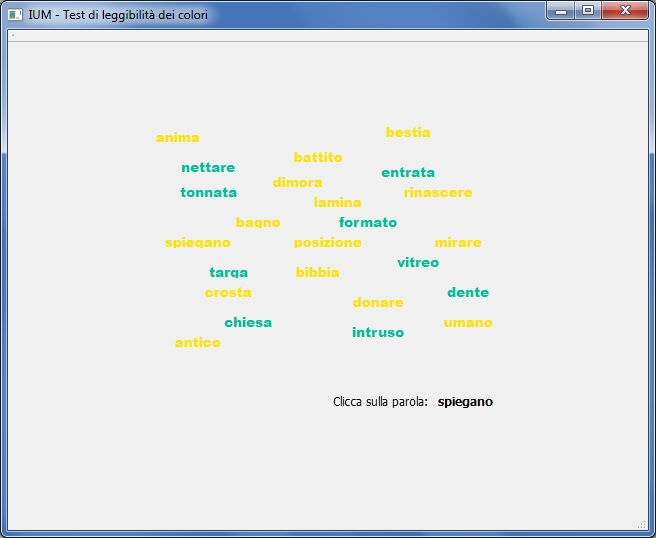
\includegraphics[width=0.7\textwidth]{dialogo2}
\caption{Un pannello del Test 1}
\label{figura:dialogo2}
\end{figure}

I colori usati nel test con relativi parametri sono riportati in tabella ~\ref{tabella:colori}.


\begin{table}[http]
\centering
\begin{tabular}{lcrrr}
\toprule
Colore & & {Hue} & {Sat} & {Val} \\
\midrule
Giallo 		& \crule[Giallo_1]{1cm}{0.3cm} & 53	& 255 & 255	\\
Azzurro	& \crule[Azzurro_1]{1cm}{0.3cm} &168	& 255	& 190	\\
\midrule
Blu 		& \crule[Blu_1]{1cm}{0.3cm} &224	& 255 & 255 \\
Rosso 	& \crule[Rosso_1]{1cm}{0.3cm} & 0	& 202	& 190	\\
\bottomrule

\end{tabular}
\caption{Specifica dei colori usati nel Test 1}
\label{tabella:colori}
\end{table}

Come si può vedere per entrambi i pannelli sono stati scelti colori con valori molto elevati sia per saturazione che per luminosità. Inoltre per ciascuna delle due combinazioni è stata mantenuta costante la differenza tra tali valori e quelli dello sfondo.
A variare notevolmente è invece la tonalità:
\begin{itemize}
\item nel primo caso sono usati \emph{giallo} e \emph{azzurro}: due colori sottrattivi chiari caratterizzati da uno scarso contrasto con lo sfondo, che quindi rendono le parole confondibili con esso;
\item nel secondo caso sono usati \emph{blu} e \emph{rosso}: due colori additivi e primari, ben distinguibili dallo sfondo, ma che rendono più difficoltosa la lettura dei caratteri. Proprio il blu e il rosso infatti, sono considerati accostati insieme i meno indicati per la leggibilità del testo. Oltre al fatto che sono entrambi saturi, il blu è da preferire per gli sfondi.
\end{itemize}

\section{Test 2}
Il Test 2 verifica la variazione di leggibilità al cambiamento dei colori di sfondo e del testo.
La sua misurazione avviene sulla base del tempo medio che le persone impiegano per leggere due predeterminati testi su schermo, il primo con un accostamento 
di colori che favorisce la lettura, il secondo con colori che rendono bassa la sua leggibilità.

Al lettore, inoltre, viene chiesto di individuare il numero di occorrenze di alcune parole, ad ogni errore commesso vengno aggiunti 500 millisecondi al tempo di lettura,
questo serve a costringere l'utente a leggere completamente il testo e quindi favorisce un esame più veritiero.

I testi sono creati senza un senso logico per evitare una interpretazione per mezzo di un meccanismo di anticipazione, attraverso il quale
un lettore immagina ciò che è scritto prima di decifrarlo, questo fatto rende i testi egualmente difficoltosi 
evitando quindi una differenza tempistica sulla base dello stile di scrittura.

L'implementazione è avvenuta mediante un \textbf{QTextBrowser} inserito in un pannello, il quale riceve, nel costruttore dell'oggetto, 
un testo formattato in HTML con annesso colore di sfondo e colore delle parole.

I vari testi dei pannelli vengono letti a partire da un file \textit{"exams.txt"} che viene inserito nell'eseguibile durante la compilazione, se necessario, 
ovviamente seguendo lo stile di formattazione del file stesso, si posso aggiungere altri testi per eseguire verifiche più accurate e/o su
altri parametri che influiscono sulla leggibilità.

\begin{figure}[http]
	\centering
	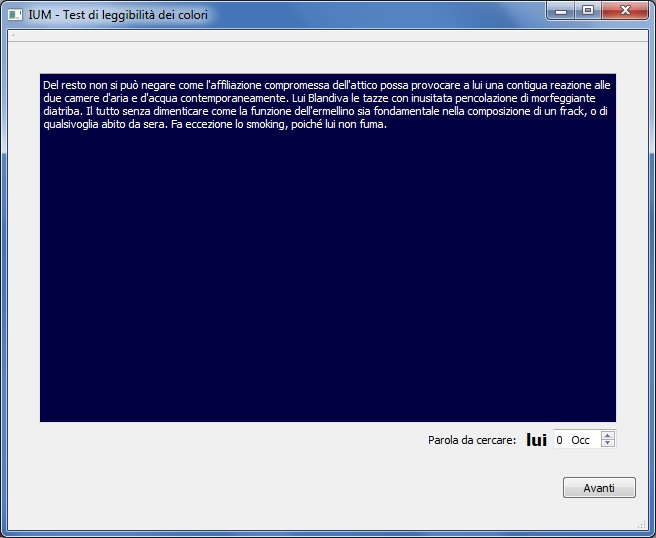
\includegraphics[width=0.65\textwidth]{dialogo1}
	\caption{Un pannello del Test 2}
	\label{figura:dialogo1}
\end{figure}

\begin{table}[http]
	\centering
  	\begin{tabular}[c]{lccrrr}
		Colore & & Posizione & Hue & Sat & Val\\
		\hline\\
		Blu Scuro & \crule[Blu_2]{1cm}{0.3cm} & Sfondo & 240 & 255 & 66\\
		Bianco & \crule[Bianco_2]{1cm}{0.3cm} & Testo & 0 & 0 & 255\\
		\\ \hline \\
		Bianco & \crule[Bianco_2]{1cm}{0.3cm} & Sfondo & 0 & 0 & 255\\
		Giallo & \crule[Giallo_2]{1cm}{0.3cm} & Testo & 60 & 255 & 212\\
	\end{tabular}
  		\caption{Colori usati nel Test2}
		\label{fig:test2_table}
\end{table}	

La tabella \ref{fig:test2_table} mostra i colori usati per il Test 2, il parametro più importate è il \textit{``val''}:
\begin{itemize}
	\item Nel primo caso il colore dello sfondo è il \textit{Blu Scuro} e il colore del testo è il \textit{Bianco}, si può notare come i due  \textit{``val''} siano molto distanti, rendendo molto leggibile il testo.
	\item Nel secondo caso il colore dello sfondo è il \textit{Bianco} a cui è stato associato, come colore delle parole, il \textit{Giallo}, due colori che hanno un \textit{``val''} molto vicino, questo rende il testo confondibile con lo sfondo  e quindi meno leggibile.
\end{itemize}


\section{Risultati}

\begin{table}[http]
\centering
\begin{tabular}{lSS}
\toprule
Run & {Test 1} & {Test 2} \\
\midrule
1971 & 203.2	& 0	\\
1976 & 289.6	& 0	\\
1986 & 812		& 0	\\
2001 & 1754.34	& 0	\\
2005 & 1824.51	& 454.62 \\
2008 & 1527.16	& 804.05 \\
2012 & 1024.94 	& 1014.61 \\
\midrule
Media & 4 & 5 \\
\bottomrule

\end{tabular}
\caption{Riepilogo dei risultati (tempi in millisecondi)}
\label{tabella:risultati}
\end{table}


\end{document}